\chapter{Обзор литературы}
\section{Приложения квантовой информатики} \label{sec:ch1/sec1}

Метод квантового распределения ключа является одним из наиболее развитых на сегодняшний день практическим приложением квантовой информатики - области знаний на стыке фотоники, теории информации и квантовой физики, которая использует квантовые биты (кубиты), то есть квантовые системы, способные находиться в двух состояниях, для осуществления передачи, хранения и обработки информации [1]. Системы квантовой коммуникации позволяют их пользователям осуществлять рассылку симметричных криптографических ключей таким образом, что любые попытки вторжения нелегитимного пользователя в канал связи принципиально обнаруживаются. К другим перспективным приложениям квантовой информатики относятся квантовый компьютер - гипотетическое вычислительное устройство, работающее на принципах квантовой механики [2] и квантовая телепортация - передача квантового состояния на расстояние [3].


В последние годы отмечается рост интереса к прикладным аспектам квантовой информатики. В частности, основными фаворитами на получение Нобелевской премии 2012 года являлись работы по открытию и экспериментальному подтверждению квантовой телепортации под авторством основоположников квантовой криптографии Ч. Беннета и Ж. Брассара [4].  


Наибольшие прикладные успехи были достигнуты именно в системах квантовой коммуникации. В последние годы успехи в разработке экспериментальных образцов этих систем сопровождаются повышением интереса к их интегрированию в волоконно-оптические линии связи, что является необходимым условием для их широкого распространения этой технологии. В мире также появились первые коммерческие образцы [5], имеется большое количество патентов на разработки в данной сфере [6,7].


На сегодняшний день исследования в области квантовой рассылки ключа находятся в экспериментальной фазе: ранее были заложены основные принципы функционирования систем, предложен ряд способов генерации и обработки квантовых состояний, разработаны протоколы генерации ключа. Сегодня разработки ведутся с целью повышения технических характеристик систем: увеличения скорости и дальности распределения ключа, повышение спектральной эффективности, уменьшения воздействия шумов и факторов внешней среды, а также их интеграции в существующие линии связи телекоммуникационного стандарта. 


\section{Системы квантовой коммуникации} \label{sec:ch1/sec2}

В современном мире требования к защите передаваемой  информации становятся все более жесткими в связи двумя проблемами:
\begin{enumerate}
	\item Условная стойкость математических алгоритмов шифрования.
Считается, что для взлома современных алгоритмов шифрования, злоумышленник не обладает достаточными вычислительными мощностями [8].
	\item Возможность появления "квантового" компьютера, обладающего необходимой вычислительной мощностью, чтобы в разумные сроки расшифровать закодированную информацию [9].
\end{enumerate} 


Наиболее выигрышную позицию в обозначенном выше вопросе занимает так называемый "метод одноразового блокнота", предложенный Г. Вернамом [10]. Идея этого метода заключается в обмене между легитимными пользователями секретными ключами, каждый из которых используется для шифрования только одного сообщения,  затем уничтожается. Для обеспечения безусловной стойкости применяют так называемый "абсолютно стойкий ключ" (АСК) [11], удовлетворяющий определенным требованиям:

\begin{enumerate}
	\item Ключ используется лишь один раз
	\item Длина ключа должна быть не менее длины шифруемого сообщения
	\item Ключ абсолютно случаен
	\item Ключ известен только легитимным пользователям
\end{enumerate}


В этих требованиях заложена проблема распространения АСК между доверенными лицами. И эту проблему можно решить, полагаясь на фундаментальные законы физики.


Итак, квантовая криптография - направление в квантовой информатике, решающее проблему распределения "абсолютно стойкого ключа" между двумя и более легитимными пользователями [12].


Уникальность этого направления заключается в том, что секретность достигается за счет фундаментальных законов квантовой механики [12, 13]. Не существует способов измерения, усиления, копирования или разделения одних параметров системы без изменения других [14]. Таким образом, на основе анализа статистики принятых отсчётов можно утверждать об отсутствии или наличии в канале связи подслушивания, неизбежно влияющего на всю систему.


Принципиальная схема системы квантовой криптографии (рис.1) включает в себя передатчик, именуемый Бобом (Bob), приёмник, именуемый Алисой (Alice), два связывающих их канала: квантовый и открытый. Также традиционно имеется нелегитимный пользователь (подслушиватель) - Ева (Eve) [12].


Принципиальная схема представлена на рис. 1
 \begin{figure}[ht]
  \centering
  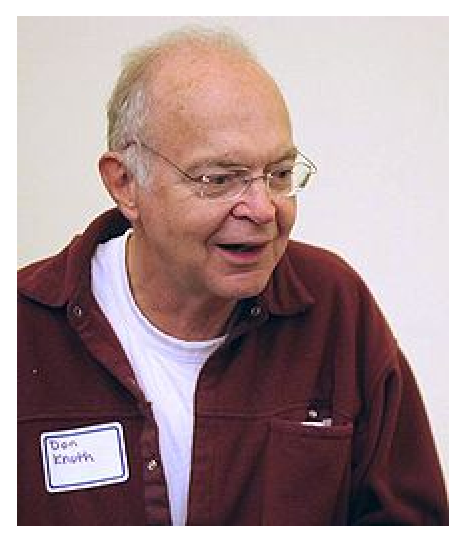
\includegraphics {knuth1}
  \caption{\todo{Принципиальная схема системы квантовой криптографии [12]}}
  \label{fig:latex}
\end{figure}


По квантовому каналу, в качестве которого используется оптоволокно, происходит распределение ключа с использованием одиночных фотонов. Открытый же канал является незащищённым и используется для выяснения легитимными пользователями изменений статистики отсчетов и коррекции ошибок в первичном ключе, переданном по квантовому каналу связи [13].




\chapter{Оформление различных элементов} \label{ch:ch1}

\section{Форматирование текста} \label{sec:ch1/sec1}

Мы можем сделать \textbf{жирный текст} и \textit{курсив}.

\section{Ссылки} \label{sec:ch1/sec2}
Сошлёмся на библиографию.
Одна ссылка: \cite[с.~54]{Sokolov}\cite[с.~36]{Gaidaenko}.
Две ссылки: \cite{Sokolov,Gaidaenko}.
Много ссылок: %\cite[с.~54]{Lermontov,Management,Borozda} % такой «фокус»
%вызывает biblatex warning относительно опции sortcites, потому что неясно, к
%какому источнику относится уточнение о страницах, а bibtex об этой проблеме
%даже не предупреждает
\cite{Lermontov, Management, Borozda, Marketing, Constitution, FamilyCode,
Gost.7.0.53, Razumovski, Lagkueva, Pokrovski, Methodology, Nasirova, Berestova,
Kriger}%
\ifnumequal{\value{bibliosel}}{0}{% Примеры для bibtex8
    \cite{Sirotko, Lukina, Encyclopedia}%
}{% Примеры для biblatex через движок biber
    \cite{Sirotko2, Lukina2, Encyclopedia2}%
}%
.
И~ещё немного ссылок:
\cite{Article,Book,Booklet,Conference,Inbook,Incollection,Manual,Mastersthesis,
Misc,Phdthesis,Proceedings,Techreport,Unpublished}
% Следует обратить внимание, что пробел после запятой внутри \cite{}
% обрабатывается ожидаемо, а пробел перед запятой, может вызывать проблемы при
% обработке ссылок.
\cite{medvedev2006jelektronnye, CEAT:CEAT581, doi:10.1080/01932691.2010.513279,
Gosele1999161,Li2007StressAnalysis, Shoji199895, test:eisner-sample,
test:eisner-sample-shorted, AB_patent_Pomerantz_1968, iofis_patent1960}
\ifnumequal{\value{bibliosel}}{0}{% Примеры для bibtex8
}{% Примеры для biblatex через движок biber
    \cite{patent2h, patent3h, patent2}%
}%
.

\ifnumequal{\value{bibliosel}}{0}{% Примеры для bibtex8
Попытка реализовать несколько ссылок на конкретные страницы
для \texttt{bibtex} реализации библиографии:
[\citenum{Sokolov}, с.~54; \citenum{Gaidaenko}, с.~36].
}{% Примеры для biblatex через движок biber
Несколько источников (мультицитата):
% Тут специально написано по-разному тире, для демонстрации, что
% применение специальных тире в настоящий момент в biblatex приводит к непоказу
% "с.".
\cites[vii--x, 5, 7]{Sokolov}[v"--~x, 25, 526]{Gaidaenko}[vii--x, 5, 7]{Techreport},
работает только в \texttt{biblatex} реализации библиографии.
}%

Ссылки на собственные работы:~\cite{vakbib1, confbib1}

Сошлёмся на приложения: Приложение \ref{app:A}, Приложение \ref{app:B2}.

Сошлёмся на формулу: формула \eqref{eq:equation1}.

Сошлёмся на изображение: рисунок \ref{fig:knuth}.

Стандартной практикой является добавление к ссылкам префикса, характеризующего тип элемента.
Это не является строгим требованием, но позволяет лучше ориентироваться в документах большого размера.
Например, для ссылок на рисунки используется префикс \textit{fig},
для ссылки на таблицу -- \textit{tab}.

В таблице \ref{tab:tab_pref} приложения \ref{app:B4} приведён список рекомендуемых
к использованию стандартных префиксов.

\section{Формулы} \label{sec:ch1/sec3}

Благодаря пакету \textit{icomma}, \LaTeX~одинаково хорошо воспринимает
в~качестве десятичного разделителя и запятую ($3,1415$), и точку ($3.1415$).

\subsection{Ненумерованные одиночные формулы} \label{subsec:ch1/sec3/sub1}

Вот так может выглядеть формула, которую необходимо вставить в~строку
по~тексту: $x \approx \sin x$ при $x \to 0$.

А вот так выглядит ненумерованая отдельностоящая формула c подстрочными
и надстрочными индексами:
\[
(x_1+x_2)^2 = x_1^2 + 2 x_1 x_2 + x_2^2
\]

При использовании дробей формулы могут получаться очень высокие:
\[
  \frac{3}{\sqrt{2}+
  \displaystyle\frac{1}{\sqrt{2}+
  \displaystyle\frac{1}{\sqrt{2}+\cdots}}}
\]

В формулах можно использовать греческие буквы:
\[
\alpha\beta\gamma\delta\epsilon\varepsilon\zeta\eta\theta\vartheta\iota\kappa%
\lambda\\mu\nu\xi\pi\varpi\rho\varrho\sigma\varsigma\tau\upsilon\phi\varphi%
\chi\psi\omega\Gamma\Delta\Theta\Lambda\Xi\Pi\Sigma\Upsilon\Phi\Psi\Omega
\]

Для красивых дробей (например, в индексах) в
\verb+userstyles.tex+ диссертации добавлен макрос
\verb+\slantfrac+, благодаря которому можно
писать $\slantfrac{1}{2}$ вместо $1/2$.

\subsection{Ненумерованные многострочные формулы} \label{subsec:ch1/sec3/sub2}

Вот так можно написать две формулы, не нумеруя их, чтобы знаки <<равно>> были
строго друг под другом:
\begin{align}
  f_W & =  \min \left( 1, \max \left( 0, \frac{W_{soil} / W_{max}}{W_{crit}} \right)  \right), \nonumber \\
  f_T & =  \min \left( 1, \max \left( 0, \frac{T_s / T_{melt}}{T_{crit}} \right)  \right), \nonumber
\end{align}

Выровнять систему ещё и по переменной $ x $ можно, используя окружение
\verb|alignedat| из пакета \verb|amsmath|. Вот так:
\[
    |x| = \left\{
    \begin{alignedat}{2}
        &&x, \quad &\text{eсли } x\geqslant 0 \\
        &-&x, \quad & \text{eсли } x<0
    \end{alignedat}
    \right.
\]
Здесь первый амперсанд (в исходном \LaTeX\ описании формулы) означает
выравнивание по~левому краю, второй "--- по~$ x $, а~третий "--- по~слову
<<если>>. Команда \verb|\quad| делает большой горизонтальный пробел.

Ещё вариант:
\[
    |x|=
    \begin{cases}
    \phantom{-}x, \text{если } x \geqslant 0 \\
    -x, \text{если } x>0
    \end{cases}
\]

Кроме того, для  нумерованых формул \verb|alignedat| делает вертикальное
выравнивание номера формулы по центру формулы. Например, выравнивание
компонент вектора:
\begin{equation}
 \label{eq:2p3}
 \begin{alignedat}{2}
{\mathbf{N}}_{o1n}^{(j)} = \,{\sin} \phi\,n\!\left(n+1\right)
         {\sin}\theta\,
         \pi_n\!\left({\cos} \theta\right)
         \frac{
               z_n^{(j)}\!\left( \rho \right)
              }{\rho}\,
           &{\boldsymbol{\hat{\mathrm e}}}_{r}\,+   \\
+\,
{\sin} \phi\,
         \tau_n\!\left({\cos} \theta\right)
         \frac{
            \left[\rho z_n^{(j)}\!\left( \rho \right)\right]^{\prime}
              }{\rho}\,
            &{\boldsymbol{\hat{\mathrm e}}}_{\theta}\,+   \\
+\,
{\cos} \phi\,
         \pi_n\!\left({\cos} \theta\right)
         \frac{
            \left[\rho z_n^{(j)}\!\left( \rho \right)\right]^{\prime}
              }{\rho}\,
            &{\boldsymbol{\hat{\mathrm e}}}_{\phi}\:.
\end{alignedat}
\end{equation}

Ещё об отступах. Иногда для лучшей <<читаемости>> формул полезно
немного исправить стандартные интервалы \LaTeX\ с учётом логической
структуры самой формулы. Например в формуле~\ref{eq:2p3} добавлен
небольшой отступ \verb+\,+ между основными сомножителями, ниже
результат применения всех вариантов отступа:
\begin{align*}
\backslash! &\quad f(x) = x^2\! +3x\! +2 \\
  \mbox{по-умолчанию} &\quad f(x) = x^2+3x+2 \\
\backslash, &\quad f(x) = x^2\, +3x\, +2 \\
\backslash{:} &\quad f(x) = x^2\: +3x\: +2 \\
\backslash; &\quad f(x) = x^2\; +3x\; +2 \\
\backslash \mbox{space} &\quad f(x) = x^2\ +3x\ +2 \\
\backslash \mbox{quad} &\quad f(x) = x^2\quad +3x\quad +2 \\
\backslash \mbox{qquad} &\quad f(x) = x^2\qquad +3x\qquad +2
\end{align*}

Можно использовать разные математические алфавиты:
\begin{align}
\mathcal{ABCDEFGHIJKLMNOPQRSTUVWXYZ} \nonumber \\
\mathfrak{ABCDEFGHIJKLMNOPQRSTUVWXYZ} \nonumber \\
\mathbb{ABCDEFGHIJKLMNOPQRSTUVWXYZ} \nonumber
\end{align}

Посмотрим на систему уравнений на примере аттрактора Лоренца:

\[
\left\{
  \begin{array}{rl}
    \dot x = & \sigma (y-x) \\
    \dot y = & x (r - z) - y \\
    \dot z = & xy - bz
  \end{array}
\right.
\]

А для вёрстки матриц удобно использовать многоточия:
\[
\left(
  \begin{array}{ccc}
    a_{11} & \ldots & a_{1n} \\
    \vdots & \ddots & \vdots \\
    a_{n1} & \ldots & a_{nn} \\
  \end{array}
\right)
\]

\subsection{Нумерованные формулы} \label{subsec:ch1/sec3/sub3}

А вот так пишется нумерованая формула:
\begin{equation}
  \label{eq:equation1}
  e = \lim_{n \to \infty} \left( 1+\frac{1}{n} \right) ^n
\end{equation}

Нумерованых формул может быть несколько:
\begin{equation}
  \label{eq:equation2}
  \lim_{n \to \infty} \sum_{k=1}^n \frac{1}{k^2} = \frac{\pi^2}{6}
\end{equation}

Впоследствии на формулы (\ref{eq:equation1}) и (\ref{eq:equation2}) можно ссылаться.

Сделать так, чтобы номер формулы стоял напротив средней строки, можно,
используя окружение \verb|multlined| (пакет \verb|mathtools|) вместо
\verb|multline| внутри окружения \verb|equation|. Вот так:
\begin{equation} % \tag{S} % tag - вписывает свой текст
  \label{eq:equation3}
    \begin{multlined}
        1+ 2+3+4+5+6+7+\dots + \\
        + 50+51+52+53+54+55+56+57 + \dots + \\
        + 96+97+98+99+100=5050
    \end{multlined}
\end{equation}

Используя команду \verb|\labelcref| из пакета \verb|cleveref|, можно
красиво ссылаться сразу на несколько формул
(\labelcref{eq:equation1,eq:equation3,eq:equation2}), даже перепутав
порядок ссылок \verb|(\labelcref{eq:equation1,eq:equation3,eq:equation2})|.
